\documentclass[a4paper,UKenglish,cleveref, autoref, anonymous, thm-restate]{lipics-v2021}
%This is a template for producing LIPIcs articles. 
%See lipics-v2021-authors-guidelines.pdf for further information.
%for A4 paper format use option "a4paper", for US-letter use option "letterpaper"
%for british hyphenation rules use option "UKenglish", for american hyphenation rules use option "USenglish"
%for section-numbered lemmas etc., use "numberwithinsect"
%for enabling cleveref support, use "cleveref"
%for enabling autoref support, use "autoref"
%for anonymousing the authors (e.g. for double-blind review), add "anonymous"
%for enabling thm-restate support, use "thm-restate"
%for enabling a two-column layout for the author/affilation part (only applicable for > 6 authors), use "authorcolumns"
%for producing a PDF according the PDF/A standard, add "pdfa"

%\pdfoutput=1 %uncomment to ensure pdflatex processing (mandatatory e.g. to submit to arXiv)
%\hideLIPIcs  %uncomment to remove references to LIPIcs series (logo, DOI, ...), e.g. when preparing a pre-final version to be uploaded to arXiv or another public repository
\usepackage{stmaryrd}
\usepackage{tikz}
\usetikzlibrary{shapes,arrows}
\usetikzlibrary{intersections}
\usetikzlibrary{automata}
\usetikzlibrary{positioning}
\usepackage{booktabs}
%\graphicspath{{./graphics/}}%helpful if your graphic files are in another directory
\usepackage{listings}
\usepackage{xcolor}

\lstdefinelanguage{SMTLIB}{
  morekeywords={set-logic, declare-fun, assert, check-sat, get-model},
  sensitive=true,
  morecomment=[l];,
  morestring=[b]"
}
\lstset{
  language=SMTLIB,
  basicstyle=\ttfamily\small,
  keywordstyle=\color{blue}\bfseries,
  commentstyle=\color{green!50!black},
  numbers=left,
  numberstyle=\tiny\color{gray},
  stepnumber=1,
  numbersep=5pt,
  backgroundcolor=\color{gray!10},
  frame=single,
  breaklines=true,
  captionpos=b,
  showstringspaces=false
}

\bibliographystyle{plainurl}% the mandatory bibstyle

\title{Certified Symbolic Transducer with Applications in String Solving} %TODO Please add

%\titlerunning{Dummy short title} %TODO optional, please use if title is longer than one line

\author{Shuanglong Kan}{Barkhausen Institut, Germany \and \url{https://github.com/ShlKan} }{shuanglongkan@gmail.com}{https://orcid.org/0000-0002-1825-0097}{(Optional) author-specific funding acknowledgements}%TODO mandatory, please use full name; only 1 author per \author macro; first two parameters are mandatory, other parameters can be empty. Please provide at least the name of the affiliation and the country. The full address is optional. Use additional curly braces to indicate the correct name splitting when the last name consists of multiple name parts.



\authorrunning{S. Kan} %TODO mandatory. First: Use abbreviated first/middle names. Second (only in severe cases): Use first author plus 'et al.'

\Copyright{Jane Open Access and Joan R. Public} %TODO mandatory, please use full first names. LIPIcs license is "CC-BY";  http://creativecommons.org/licenses/by/3.0/

\ccsdesc[100]{\textcolor{red}{Replace ccsdesc macro with valid one}} %TODO mandatory: Please choose ACM 2012 classifications from https://dl.acm.org/ccs/ccs_flat.cfm 

\keywords{Dummy keyword} %TODO mandatory; please add comma-separated list of keywords

\category{} %optional, e.g. invited paper

\relatedversion{} %optional, e.g. full version hosted on arXiv, HAL, or other respository/website
%\relatedversiondetails[linktext={opt. text shown instead of the URL}, cite=DBLP:books/mk/GrayR93]{Classification (e.g. Full Version, Extended Version, Previous Version}{URL to related version} %linktext and cite are optional

%\supplement{}%optional, e.g. related research data, source code, ... hosted on a repository like zenodo, figshare, GitHub, ...
%\supplementdetails[linktext={opt. text shown instead of the URL}, cite=DBLP:books/mk/GrayR93, subcategory={Description, Subcategory}, swhid={Software Heritage Identifier}]{General Classification (e.g. Software, Dataset, Model, ...)}{URL to related version} %linktext, cite, and subcategory are optional

%\funding{(Optional) general funding statement \dots}%optional, to capture a funding statement, which applies to all authors. Please enter author specific funding statements as fifth argument of the \author macro.

\acknowledgements{I want to thank \dots}%optional

%\nolinenumbers %uncomment to disable line numbering



%Editor-only macros:: begin (do not touch as author)%%%%%%%%%%%%%%%%%%%%%%%%%%%%%%%%%%
\EventEditors{John Q. Open and Joan R. Access}
\EventNoEds{2}
\EventLongTitle{15th Conference on
Interactive Theorem Proving (ITP 2025)}
\EventShortTitle{ITP 2025}
\EventAcronym{ITP}
\EventYear{2025}
\EventDate{July 24--27, 2025}
\EventLocation{Little Whinging, United Kingdom}
\EventLogo{}
\SeriesVolume{42}
\ArticleNo{23}
%%%%%%%%%%%%%%%%%%%%%%%%%%%%%%%%%%%%%%%%%%%%%%%%%%%%%%

\lstset{
	basicstyle=\ttfamily,
	keywordstyle=\color{blue}\bfseries,
	keywords={definition,if,then,else, where, record, fun, lemma, type_synonym, fixes, shows, assumes, shows},
	escapeinside={|}{|}
}

\begin{document}

\maketitle

%TODO mandatory: add short abstract of the document
\begin{abstract}
Finite-state Automata (FAs) are fundamental components in the domains of programming languages. For instance, regular expressions, which are pivotal in languages such as JavaScript and Python, are frequently implemented using FAs.
%
Finite-state Transducers (FTs) extend the capabilities of FAs by enabling the transformation of input strings into output strings, thereby providing a more expressive framework for operations that encompass both recognition and transformation. Despite the widespread adoption of formalizing FAs and FTs within proof assistants such as Coq and Isabelle/HOL, these formalizations often fall short in terms of applicability to real-world scenarios. A significant limitation of classical finite-state models is that transition labels are typically confined to a single character from a finite alphabet. However, in practical applications, the alphabet of an FA or FT can be extensive or even \emph{infinite}. This classical approach to formalizing transitions can result in transition explosion, leading to critical performance bottlenecks of FA operations.

A more pragmatic approach involves the formalization of symbolic FAs \cite{cav/DAntoniV17} and FTs \cite{VeanesHLMB12Transducer}, where transition labels are symbolic and potentially infinite. While the formalization of symbolic FAs has been explored in the work of CertiStr \cite{cpp/KanLRS22}, the formalization of symbolic FTs in interactive proof assistants remains largely unexplored due to the increased complexity challenges.
%
In this paper, we aim to formalize symbolic FTs within the Isabelle/HOL framework. This formalization is refinement-based and is designed to be extensible with various symbolic representations of transition labels. To assess its performance, we applied the formalized symbolic FTs to an SMT string solver for modeling replacement operations. The experimental results indicate that the formalized symbolic transducer can efficiently solve string constraints.


\end{abstract}

\section{Introduction}
\label{sec:introduction}

Finite-state Automata (FA) and Finite-state Transducers (FT) are fundamental constructs in the theory of formal languages, with extensive applications in programming languages and software engineering. For example, recent advancements in string solvers, as demonstrated by \cite{pacmpl/ChenFHHHKLRW22}, have illustrated the relationship between regular expressions in modern programming languages and various forms of FAs and FTs. Additionally, FAs and FTs find significant industrial applications, such as in the verification of AWS access control policies \cite{DBLP:conf/fmcad/BackesBCDGLRTV18}.


Even though there are various formalizations of FAs and FTs in interactive proof assistants such as Isabelle \cite{isabelle-homepage} and Coq \cite{coq-homepage}, these are predominantly based on classical definitions. However, these traditional approaches present certain limitations when applied to practical scenarios. One significant drawback is that transition labels are typically non-symbolic and finite. A conventional transition is represented as $q\xrightarrow{a}q'$, where $a$ is a character from a finite alphabet. This simplistic representation can lead to a phenomenon known as transition explosion. For example, if the alphabet $\Sigma$ encompasses the entire Unicode range, which is common in modern programming languages, it consists of $\texttt{0x10FFFF}$ distinct characters. Defining a transition from state $q$ to $q'$ that accepts any character in $\Sigma$ would require splitting into $\texttt{0x10FFFF}$ individual transitions, rendering the product of two FAs highly inefficient. Furthermore, in practical applications, it is often necessary to consider infinite alphabets, such as the set of all integers.



Symbolic Finite Automata (SFA) and Symbolic Finite-state Transducers (SFT) \cite{cav/DAntoniV17, VeanesHLMB12Transducer} represent advanced extensions of classic Finite Automata (FAs) and Finite-state Transducers (FTs), enhancing their applicability in practical scenarios. These symbolic models utilize transition labels defined by boolean algebras, allowing for more expressive representations. For example, a transition label might be specified as an interval ($'\texttt{a}'-'\texttt{z}'$), encompassing all characters from $'\texttt{a}'$ to $'\texttt{z}'$, or as an arithmetic condition ($x \% 2 = 0$), denoting all even numbers. This symbolic approach not only provides a more succinct representation but also supports infinite alphabets, thereby extending the expressive capabilities of FAs and FTs.


The formalization of transition labels in SFAs and SFTs presents significant challenges within interactive proof assistants. Two fundamental considerations arise: first, the representation of transition labels must be sufficiently expressive to accommodate diverse boolean algebras; second, the formalization framework must be designed with extensibility in mind to facilitate the incorporation of new boolean algebras while minimizing redundant proof efforts.




Prior work has successfully formalized symbolic FAs within Isabelle/HOL through CertiStr \cite{cpp/KanLRS22}, demonstrating both the efficiency and effectiveness of symbolic FAs in practice. However, the formalization of FTs remains an open challenge, primarily due to their inherent complexity in two aspects: the formalization of transition labels and the specification of transition output functions. FTs constitute a significantly more expressive and powerful theoretical framework compared to symbolic FAs, as evidenced by their capability to model complex string transformations such as replacement operations.
Furthermore, the seminal work of \cite{VeanesHLMB12Transducer} demonstrates the broad applicability of SFTs across diverse domains, including security-critical applications such as cross-site scripting (XSS) prevention, image transformation operations, and privacy-preserving location data processing.


 
In this work, we present a comprehensive formalization of symbolic FTs that builds upon the formalization of symbolic FAs. To address the extensibility challenges inherent in supporting diverse transition label theories, we adopt a refinement-based approach. At the abstraction level, transition labels are formalized through the fundamental mathematical concept of \emph{sets}. This abstraction facilitates subsequent refinement to various boolean algebras, including intervals and arithmetic conditions, while maintaining theoretical consistency.

The key operation of our formalization is the product operation between an SFT and an input regular language. Specifically, given an SFA $\mathcal{A}$ representing a regular language and an SFT $\mathcal{T}$, we define the product operation $\mathcal{T} \times\mathcal{A}$ that characterizes the set of output languages generated by $\mathcal{T}$ when processing inputs from the language recognized by $\mathcal{A}$.


Leveraging the data refinement framework \cite{DBLP:conf/itp/Lammich13} formalized in Isabelle/HOL, we implement an efficient representation of states and transitions using sophisticated data structures such as hashmaps and red-black trees. Furthermore, we develop a comprehensive interval algebra that provides efficient operations for creation, verification, and manipulation of intervals, thereby facilitating the implementation of replacement operations within our string solver framework. 


In summary, Our formalization makes two primary contributions. First, we achieve computational efficiency through an algebraic representation that enables compressed storage of transition labels. Second, our refinement-based formalization framework demonstrates significant extensibility, facilitating the incorporation of diverse theories of transition labels.



The paper is organized as follows.
Section \ref{sec:formalization} presents the formalization of symbolic FTs.
Section \ref{sec:product-operation} presents the product operation of symbolic FTs in the abstraction level.
Section \ref{sec_alg_refinement} presents the refinement of the product operation in Isabelle/HOL.
Section \ref{sec-app-str-solver} presents the application of SFTs in the modeling of replacement operations in string solvers.
Section \ref{sec:related-work} presents the related work.
Section \ref{sec:conclusion} concludes the paper. 




\section{Formalization of Symbolic FTs}
\label{sec:formalization}


We begin by presenting a mathematical definition of SFTs \cite{VeanesHLMB12Transducer}, abstracting from the specific implementation details of Isabelle/HOL. The foundational concept underlying this formalization is the label theory, which characterizes the process by which output labels are derived from input labels.


Let $\mathcal{U}$ be a multi-sorted carrier set or background universe, which is equipped with functions and relations over the elements. We use $\tau$ as a sort and $\mathcal{U}^\tau$ denotes the sub-universe of elements of type $\tau$. 
We have a special type $\mathbb{B}$ with $\mathcal{U}^\mathbb{B} = \{ \top, \bot\}$, which corresponds to the boolean type. 

A lambda term is defined as $\lambda x.~t$ of type $\tau_1 \rightarrow \tau_2$.
When $\tau_2$ is $\mathbb{B}$, this lambda term is a predicate. Let $\phi$ be a predicate. We write $a\in \llbracket\phi \rrbracket$ if $\phi~a=\top$. For non-predicate lambda terms, we view them as functions that generate output elements of type $\tau_2$ given input terms of type $\tau_1$. 
With these notations and the above definitions, we can define SFTs as follows.

\begin{definition}[Symbolic Finite Transducer]
\label{def-sft}
   A Symbolic Finite Transducer over $\tau_1\rightarrow \tau_2$ is a quadruple $\mathcal{T} = (\mathcal{Q}, \Delta, \mathcal{I}, \mathcal{F})$, where 
   \begin{itemize}
   \item $\mathcal{Q}$ is a finite set of states,
   \item $\mathcal{I}\subseteq \mathcal{Q}$ is the set of initial states,
   \item $\mathcal{F} \subseteq\mathcal{Q}$ is the set of accepting states,
   \item $\Delta$ is the set of transition relations. Each element in $\Delta$ is of the form $(q, \phi, f, q')$ or written as $q\xrightarrow{\phi, f} q'$, where $q$ and $q'$ are states in $\mathcal{Q}$.
   $\phi$ is a predicate of type $\tau_1\rightarrow \mathbb{B}$.
   $f$ is a lambda term of type $\tau_1\rightarrow \tau_2$. $f$ is called an \emph{output function}.
   \end{itemize}

For each transition $q\xrightarrow{\phi, f} q'$, if there exists an element $a\in \llbracket \phi \rrbracket$, where $a$ is called an input,  then the application $(f~a)$ is the output.
   
\end{definition}

SFTs accept an input word and generate an output. This can be defined by \emph{runs} of SFTs.
An SFT run $\sigma$ is a sequence $(q_0, \phi_0, f_0, q_1),(q_1, \phi_1, f_1, q_2),\ldots, (q_{n-1}, \phi_{n-1}, f_{n-1}, q_n)$ such that $q_0\in \mathcal{I}$ and $(q_i, 
\phi_i, f_i, q_{i+1}), 0 \leq i \leq n-1$ is a transition in $\Delta$.
$\sigma$ is an accepting run when $q_n$ is an accepting state.

For a word $w = a_0,\ldots, a_{n-1}$, it is accepted by $\sigma$ if and only if $a_i \in \llbracket\phi_i \rrbracket$ for $0 \leq i \leq n - 1$. When $w$ is accepted, run $\sigma$ generates an output sequence $w'= f_0~a_0, \ldots, f_{n-1}~a_{n-1}$. We define:
\begin{itemize}
\item  $(a_0,(f_0~a_0)), \ldots, (a_{n-1},(f_{n-1}~a_{n-1}))$ a \emph{trace},
\item $a_0,\ldots,a_{n-1}$ the \emph{input} of the trace and $(f_0~a_0), \ldots, (f_{n-1}~a_{n-1})$ the \emph{output} of the trace.
\end{itemize}

If $a_0,\ldots,a_{n-1}$ is accepted by an accepting run in $\mathcal{T}$, we say that the trace is an accepting trace of $\mathcal{T}$.
For a trace $\pi$, we denote its input as $\mathit{in}(\pi)$ and its output as $\mathit{out}(\pi)$.
%
Given an SFT $\mathcal{T}$ and a word $w$, we define the \emph{product} operation of $\mathcal{T}$ and $w$ (denoted as $\mathcal{T}\times\{w\}$) as the set of outputs generated by $\mathcal{T}$ with input $w$. More precisely, 
\[
\mathcal{T}\times\{w\} = \{w'\mid \exists \pi.~\pi \text{ is an accepting trace of } \mathcal{T} \land in(\pi) = w \land out(\pi) = w'\}.
\]

To make the operation \emph{product} more general, we extend the operation to an SFT and a set of input words represented by a regular language, which can be denoted by an NFA $\mathcal{A}$. More precisely,
\[
\mathcal{T}\times \mathcal{A} = \{w'\mid \exists w.~w\in \mathcal{L}(\mathcal{A})\land w' \in \mathcal{T}\times\{w\}\}, \text{ where }\mathcal{L}(\mathcal{A})\text{ denotes the language of }\mathcal{A}.
\] 

\begin{figure}[hbt!]
  \centering
  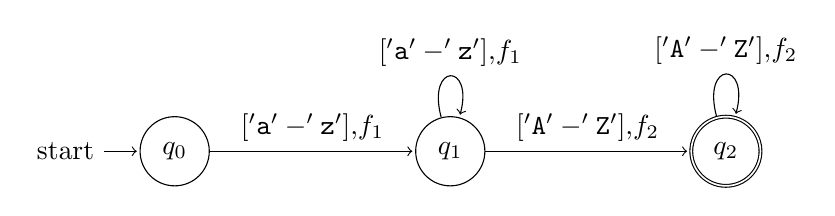
\begin{tikzpicture}[shorten >=1pt, node distance=3.5cm, on grid, auto]
    \node[state, initial] (q_0)   {$q_0$}; 
    \node[state] (q_1) [right=of q_0] {$q_1$}; 
    \node[state, accepting] (q_2) [right=of q_1] {$q_2$}; 
 
    \path[->] 
    (q_0) edge node {[$'\texttt{a}'-'\texttt{z}'$],$f_1$} (q_1)
    (q_1) edge node {[$'\texttt{A}'-'\texttt{Z}'$],$f_2$} (q_2)
    (q_1) edge[loop above] node {[$'\texttt{a}'-'\texttt{z}'$],$f_1$} (q_1)
    (q_2) edge[loop above] node {[$'\texttt{A}'-'\texttt{Z}'$],$f_2$} (q_2);
 \end{tikzpicture}
    \caption{An example of SFT}
    \label{fig-example-ft}
    \end{figure}   

    Figure \ref{fig-example-ft} illustrates an SFT that accepts strings matching the regular expression $/['\texttt{a}'-'\texttt{z}']+['\texttt{A}'-'\texttt{Z}']+/$. The transition labels utilize intervals of the form $[i\text{-}j]$, which are interpreted as predicates $\lambda x.~i \leq x \leq j$. The output functions $f_1$ and $f_2$ perform case transformations: $f_1 = \lambda x.~\texttt{toUpper}(x)$ converts lowercase letters to uppercase, while $f_2 = \lambda x.~\texttt{toLower}(x)$ performs the inverse operation. For example, given the input string \texttt{"bigSMALL"}, this SFT produces the output \texttt{"BIGsmall"}.


%The transition labels can be more complex. For instance, it can be a predicate over integers as: $\lambda x.~ x >0 \land x \text{ mod } 2 = 0$. This symbolic label corresponds to the set of even natural numbers.





\subsection{The Isabelle/HOL Formalization of SFTs}

As we have discussed the diversity of transition labels in Section \ref{sec:introduction}, we now present an extensible formalization of SFTs that accommodates this variety. Our approach leverages the refinement framework (Refine\_Monadic \cite{Refine_Monadic-AFP}) in Isabelle/HOL to achieve the flexibility and extensibility of transition labels modeling.

\begin{figure}[hbt!]
	\begin{lstlisting}
record (|$'q,$||$~'a,$| |$'b$|) |$\texttt{NFT}$| =
	|$\mathcal{Q}_t$| :: "|$'q$| set"
	|$\Delta_t$| :: "(|$'q,$||$~'a,$| |$'b$|) LTTS"
	|$\mathcal{I}_t$| :: "|$'q$| set"
	|$\mathcal{F}_t$| :: "|$'q$| set"
        |$\mathcal{M}_t$| :: "|$'b\Rightarrow 'a$| Tlabel"
        
type_synonym |$('q, 'a, 'b)$| LTTS = "|$('q \times ('a \text{ set option }\times b) \times 'q)$| set"

type_synonym |$'a$| Tlabel = "|$'a \text{ option}~\Rightarrow~'b$ set option"
	\end{lstlisting}
\caption{The formalization of $FTs$ in Isabelle/HOL}
\label{fig-def-FT}
\end{figure}

Figure \ref{fig-def-FT} presents our formalization of SFTs in Isabelle/HOL. While the elements $\mathcal{Q}_t$, $\mathcal{I}_t$, and $\mathcal{F}_t$ directly correspond to their counterparts ($\mathcal{Q}$, $\mathcal{I}$, and $\mathcal{F}$) in Definition \ref{def-sft}, the transition relations are not exactly the same.
%
The transition relations are formalized through \texttt{LTTS} (Labeled Transducer Transition System), where each transition is represented as a triple $'q \times ('a \text{ set option }\times b) \times 'q$. This representation reflects several key design decisions aimed at enhancing the abstraction and flexibility of our SFT formalization.


Firstly, $'a \text{ set option }$ is the input type of the transition, it accepts a set of elements of type $'a$ or $\texttt{None}$ corresponding to empty string $\varepsilon$. 
Accepting a set of $'a$ elements aims to express the same but more abstract semantics of the input labels in Definition \ref{def-sft}, in which an input label is a predicate. A predicate's semantics as introduced before represents a set of elements that make the predicate true. But predicates have various different forms. For instance, the interval $[1, 9]$ represents the set $\{e \mid 1 \leq e \leq 9\}$. The predicate $\lambda x \colon \mathbb{N}.~ x \text{ mod } 2 = 0$ denotes the set of even natural numbers. All these different forms of labels are abstracted as sets in our formalization.
%
The value $\texttt{None}$ represents the empty string $\varepsilon$ in our formalization, indicating a transition that consumes no input but may still produce output elements. This design choice facilitates the modeling of real-world applications in SFTs, as we will demonstrate in our application to string solvers.

The second element of type $'b$ serves as an index into the output function space. The mapping $\mathcal{M}_t$ associates each index with a specific output function. These output functions, formalized by \texttt{Tlabel}, map a single input element to a set of possible output elements rather than to a single element. This design enables non-deterministic output behavior, where the transducer may select any element from the output set randomly or according to specified criteria. Additionally, output functions can produce the empty string $\varepsilon$ by returning $\texttt{None}$, providing further flexibility in transition behavior.

%Now let us look at an example. In some modern programming languages, there are support for replacement operations : $\texttt{replace}(\texttt{str}, \texttt{pattern}, \texttt{replacement})$. This operation replaces the first occurrence of the substring  in \texttt{str} that matches \texttt{pattern} (which usually a regular expression) with the string \texttt{replacement}). 
%We can easily model this operation using our formalization of NFTs with the following steps:
%\begin{itemize}
%\item Step 1, construct a corresponding NFA from \texttt{pattern}).
%\item Step 2, convert each transition label for transducers by adding a function that maps each input character to empty, that is, generate nothing.
%\item Step 3, Add a new accepting state, and redirect existing accepting states to the new accepting state and transition label as $(\texttt{None}, \lambda x. \texttt{replacement})$.
%\item Step 4, unlabel previous accepting states as non-accepting states. 
%\end{itemize}

%We can see that the definition of transition labels in NFTs makes it is very easy to model the replacement operation.

\section{The Product Operation of NFTs}
\label{sec:product-operation}

In this section, we formalize the product operation between an SFT $\mathcal{T}$ and an SFA $\mathcal{A}$, denoted as $\mathcal{T} \times \mathcal{A}$ in Section \ref{sec:formalization}. An additional consideration in this operation is the presence of $\varepsilon$-transitions in our SFT formalization, which implies that the resulting automata may also contain $\varepsilon$-transitions. Since CertiStr \cite{cpp/KanLRS22} does not include a formalization of automata with $\varepsilon$-transitions ($\varepsilon$NFAs), we extend the framework with a formalization of symbolic $\varepsilon$NFAs (denoted as $\varepsilon$SFA) and provide a verified conversion to standard SFAs. In this paper, we present only the definitions of  $\varepsilon$SFAs and SFAs, while the complete formalization, including correctness proofs, is available in our Isabelle development.

\begin{figure}[hbt!]
	\begin{lstlisting}
record (|$'q,$||$~'a$|) |$\texttt{NFA}$| =
	|$\mathcal{Q}$| :: "|$'q$| set"
	|$\Delta$| :: "(|$'q,$||$~'a$|) LTS"
	|$\mathcal{I}$| :: "|$'q$| set"
	|$\mathcal{F}$| :: "|$'q$| set"

record (|$'q,$||$~'a$|) |$\texttt{eNFA}$| =
	|$\mathcal{Q}_e$| :: "|$'q$| set"
	|$\Delta_e$| :: "(|$'q,$||$~'a$|) LTS"
	|$\Delta_e'$| :: "|$('q * 'q)$| set"
	|$\mathcal{I}_e$| :: "|$'q$| set"
	|$\mathcal{F}_e$| :: "|$'q$| set"

type_synonym |$('q, 'a)$| LTS = "|$'q \times 'a \text{ set }\times 'q$|"    
	\end{lstlisting}
\caption{The formalization of $\varepsilon$NFA and SFA in Isabelle/HOL}
\label{fig-def-FAs}
\end{figure}

Figure \ref{fig-def-FAs} presents the formalization of both SFAs and $\varepsilon$SFAs using Isabelle/HOL record types \texttt{NFA} and \texttt{eNFA}, respectively. The $\varepsilon$SFA formalization extends the standard SFA structure by introducing $\Delta_e'$, which captures $\varepsilon$-transitions as pairs of states, while maintaining the same labeled transition relation $\Delta$ as in standard SFAs.

Having established these foundational definitions, we can now formalize the product operation. 

\begin{figure}[hbt!]
	\begin{lstlisting}
definition productT :: |$"('q,'a,'b,'c)"$| NFT |$\Rightarrow$| ('q,'a) NFA |$\Rightarrow$| 
           |$(('a,'b)$| Tlabel |$\Rightarrow 'a \text{ set}\Rightarrow 'b\text{ set option})\Rightarrow$|
           |$('q\times 'q, ~'b)$| eNFA where
  "productT |$\mathcal{T}$| |$\mathcal{A}$| F = |$\llparenthesis$|
    |$\mathcal{Q}e = \mathcal{Q}_t~\mathcal{T} \times \mathcal{Q} ~\mathcal{A}$|,
    |$\Delta_e = \{((p,p'),~\texttt{the }(((\mathcal{M}~\mathcal{T})~f)\texttt{ None}),~(q, p'))\mid p, p', q, f.~p'\in \mathcal{Q}~\mathcal{A} \land$|
          |$(p, (\texttt{None}, f), q)\in \Delta_T \mathcal{T} \land \exists S. (\mathcal{M}~\mathcal{T})~f~\text{None} = \text{Some } S\} ~\cup$|
        |$\{((p,p'),~\texttt{the }(F~((\mathcal{M}~\mathcal{T})~f)~(\sigma_1\cap\sigma_2)),~(q, q'))\mid p, p', q, \sigma_1, \sigma_2, q', f.~$|
          |$ (p, (\text{Some }\sigma_1, f), q)\in \Delta_T~\mathcal{T} \land (p', \sigma_2, q')\in\Delta~\mathcal{A}\land \sigma_1\cap \sigma_2 = \emptyset \land$|
            |$ \exists S.~F~((\mathcal{M}~\mathcal{T})~f)~(\sigma_1\cap\sigma_2) = \text{Some } S\}$|,
    |$\Delta_e' = \{((p,p'),~\text{the }(((\mathcal{M}~\mathcal{T})~f)\texttt{ None}),~(q, p'))\mid p, p', q, f.~p'\in \mathcal{Q}~\mathcal{A} \land$|
          |$(p, (None, f), q)\in \Delta_T~\mathcal{T} \land (\mathcal{M}~\mathcal{T})~f~\texttt{None} = \text{None}\} ~\cup$|
        |$\{((p,p'),~\texttt{the }(F~((\mathcal{M}~\mathcal{T})~f)~(\sigma_1\cap\sigma_2)),~(q, q'))\mid p, p', q, \sigma_1, \sigma_2, q', f.~$|
          |$ (p, (\text{Some }\sigma_1, f), q)\in \Delta_T~\mathcal{T} \land (p', \sigma_2, q')\in\Delta~\mathcal{A}\land \sigma_1\cap \sigma_2 = \emptyset \land$|
            |$ \exists x\in(\sigma_1\cap\sigma_2).~((\mathcal{M}~\mathcal{T})~f)~(\text{Some } x) = \text{None} \}$|,
    |$\mathcal{I}_e = \mathcal{I}_t~\mathcal{T} \times \mathcal{I}~\mathcal{A}$|
    |$\mathcal{F}_e = \mathcal{F}_t~\mathcal{T} \times \mathcal{F}~\mathcal{A}$| |$\rrparenthesis$|"
	\end{lstlisting}
\caption{The formalization of $\varepsilon-$NFA and NFA in Isabelle/HOL}
\label{fig-def-FTProd}
\end{figure}

Figure \ref{fig-def-FTProd} depicts the abstract level formalization for the product of an SFT and an SFA. The parameters $\mathcal{T}$ and $\mathcal{A}$ are an SFT and an SFA, respectively. But we need to explain the role of $\text{\texttt{F}}$. The output function $f$ for each transition in $\Delta_t$ is of type "$'a\;\text{option} \Rightarrow 'b\;\text{set option}$", which applies to a \emph{single} element of type $'a$ or $\varepsilon$. $\text{\texttt{F}}$ extends $f$ to apply it to a set of elements. More precisely, let $f$ be an output function, the semantics of $\text{\texttt{F}}$ is defined as 

\[\texttt{F}~f~A=\bigcup_{a\in A} (\text{if }f~a= \text{Some }S \texttt{ then } S \texttt{ else } \emptyset)\].

The transition relations $\Delta_e$ and $\Delta_e'$ are determinted by considering two distinct cases based on the nature of transitions in the SFT: $\varepsilon$-transitions and non-$\varepsilon$-transitions. In both cases, the transition labels in the resulting $\varepsilon$SFA are derived from the composition of the SFT's output function and the SFA's input labels:
For transitions in $\Delta_e$, 

\begin{enumerate}
\item When $(p, (\text{None}, f), q)$ is a transition in $\Delta_t$, the input character is $\varepsilon$. Consequently, the SFA remains in its current state, and the product transition produces the output $(f~\text{None})$.

\item When $(p, (\text{Some}~\sigma_1, f), q)$ is a transition in $\Delta_t$, synchronization is possible only with SFA transitions that share characters with $\sigma_1$. The resulting output is $F~f~(\sigma_1\cap\sigma_2)$, where $\sigma_2$ represents the input label of the corresponding SFA transition.
\end{enumerate}

The transitions in $\Delta_e'$ follow a similar pattern with analogous cases for $\varepsilon$ and non-$\varepsilon$ transitions.

To establish the correctness specification of the product operation, we begin by formalizing the concept of SFT \emph{traces} as introduced in Definition \ref{def-sft}. In our formalization, traces are represented by the type $('a\;\text{option} \times 'b\;\text{option})\;\texttt{list}$, as shown in Figure \ref{fig-def-output}.
%
Given a trace $\pi$, we define two key projection functions:
(1) \texttt{inputE}, which corresponds to $\text{in}(\pi)$ and extracts the input sequence
(2) \texttt{outputE}, which corresponds to $\text{out}(\pi)$ and extracts the output sequence.

The definition \texttt{outputL} generalizes \texttt{outputE} to characterize the set of all possible outputs that an SFT $\mathcal{T}$ can generate when processing inputs from the language accepted by the SFA $\mathcal{A}$. The reachability of a trace $\pi$ between states $q$ and $q'$ in an SFT $\mathcal{T}$ is verified by the predicate $\texttt{LTTS\_reachable}~\Delta_t~M~q~\pi~q'$.





\begin{figure}[hbt!]
	\begin{lstlisting}
fun inputE :: |$('a\;\text{option}\;\times\;'b\;\text{option})\;\text{list}\;\Rightarrow\;'a\;\text{list}$| where
  "inputE [] = []" |$\mid$|
  "inputE ((Some a, |$\_$|) |$\#$| l) = a |$\#$| (inputE l)" |$\mid$|
  "inputE ((None, |$\_$|) |$\#$| l) = (inputE l)"

fun outputE :: "|$('a \text{ option} \times 'b \text{ option}) \text{ list} \Rightarrow 'b \text{ list}$|" where
  "outputE [] = []" |$\mid$|
  "outputE ((_, Some a) # l) = a # (outputE l)" |$\mid$|
  "outputE ((_, None) # l) = (outputE l)"

definition outputL :: "|$('q, 'a, 'b, 'c)\text{  NFT} \Rightarrow $|
            |$ ('c \Rightarrow ('a, 'b)\text{  Tlabel}) \Rightarrow 
                               ('q, 'a) \text{ NFA\_rec} \Rightarrow 'b\text{ list set}$|" where
  "outputL |$\mathcal{T}$| M |$\mathcal{A}$| = {outputE |$\pi~\mid~\pi~q~q'$|. |$q\in \mathcal{I}_t~\mathcal{T} \land q' \in \mathcal{F}_t~\mathcal{T} \land$|
                |$ \text{LTTS\_reachable }(\Delta_t~\mathcal{T})~\text{M}~q~\pi~q'\land \text{inputE }\pi\in \mathcal{L}~\mathcal{A}$|}" 
	\end{lstlisting}
\caption{The formalization of $\varepsilon-$NFA and NFA in Isabelle/HOL}
\label{fig-def-output}
\end{figure}


\begin{figure}[hbt!]
	\begin{lstlisting}
lemma productT_correct:
  fixes |$\mathcal{T}$| |$\mathcal{A}$| F
  assumes F_ok1: "|$\forall~f~s.~(\forall e \in s. f (\text{ Some } e) = \text{None}) \mapsto \text{ F}~f~s = \text{None}"$|
      and F_ok2: "|$\forall~f~s.~\text{F }f~s = $|
            |$\text{Some }(\cup \{\text{the }(f (\text{ Some }e))\mid e. e \in s \land f~(\text{Some }e) \neq \text{ None}\})$|"
      and wfTA: "NFT_wf |$\mathcal{T}~\land \text{ NFA } \mathcal{A}$|"
    |$\textcolor{blue}{\text{shows}}$| "|$\mathcal{L}_e$| (productT |$\mathcal{T}~\mathcal{A}$| F) = outputL |$\mathcal{T}~(\mathcal{M}~\mathcal{T})~\mathcal{A}$|"

	\end{lstlisting}
\caption{The formalization of $\varepsilon-$NFA and NFA in Isabelle/HOL}
\label{fig-def-product-correct}
\end{figure}

Figure \ref{fig-def-product-correct} presents Lemma \texttt{productT\_correct}, which establishes the correctness of the product operation. The lemma's assumptions, \texttt{F\_ok1} and \texttt{F\_ok2}, specify the essential properties of function \texttt{F}. The conclusion, marked by \textcolor{blue}{\texttt{shows}}, demonstrates that the language of the constructed $\varepsilon$SFA ($\mathcal{L}_e$ denotes the language of $\varepsilon$SFA) from $\mathcal{T} \times \mathcal{A}$ coincides with the mathematical semantics defined by \texttt{outputL}, thereby establishing semantic preservation of the product construction.

\section{Algorithm Level Refinement}
\label{sec_alg_refinement}
Having established the abstract definition of the SFT product operation in Section \ref{sec:product-operation}, we now present its algorithmic refinement. This section introduces an efficient implementation of the product construction and refines the abstract representation of transition labels to a concrete interval algebra, enabling practical computation.


\subsection{Intervals}

An interval is defined as a pair $(i, j)$ representing the set $\{e \mid i \leq e \leq j\}$. To achieve greater expressiveness, our formalization extends this notion to interval lists of the form $[(i_1, j_1), \ldots, (i_n, j_n)]$, which denote the set $\bigcup_{1\leq k\leq n}\{e \mid i_k \leq e \leq j_k\}$. This generalization offers two key advantages: it enables more compact representation of transitions in SFAs and SFTs through merging, and it allows for efficient handling of interval operations without unnecessary splitting. For example, the set difference between intervals $[1, 5]$ and $[3, 4]$ can be directly represented as the interval list $[(1, 2), (5, 5)]$.


Throughout the following discussion, we use the term "interval" to refer to interval lists. Our formalization provides a collection of interval operations through the following interface:

\begin{enumerate}
  \item $\texttt{semI}~i$: Defines the semantic interpretation of an interval as a set. For an interval $(i,j)$, $\texttt{semI}~(i,j) = \{e \mid i \leq e \leq j\}$.
  \item $\texttt{emptyI}~i$: Tests whether an interval represents an empty set, i.e., whether $\texttt{semI}~i = \emptyset$.
  \item $\texttt{nemptyI}~i$: Tests whether an interval represents a non-empty set, i.e., whether $\texttt{semI}~i \neq \emptyset$.
  \item $\texttt{intersectIs}~i_1~i_2$: Computes the intersection of two intervals, yielding an interval $i$ such that $\texttt{semI}~i = \texttt{semI}~i_1 \cap \texttt{semI}~i_2$.
  \item $\texttt{diffIs}~i_1~i_2$: Computes the set difference of two intervals, yielding an interval $i$ such that $\texttt{semI}~i = \texttt{semI}~i_1 \setminus \texttt{semI}~i_2$.
\end{enumerate}


To facilitate formal reasoning and optimize performance, we introduce a canonical form for interval. An interval $[(i_1, j_1), \ldots, (i_n, j_n)]$ is in canonical form if it satisfies two key properties:
\begin{enumerate}
  \item Each $(i_k, j_k)$ is well-formed: $i_k \leq j_k$ for all $k \in \{1,\ldots,n\}$
  \item Intervals are ordered and non-overlapping: $j_k < i_{k+1}$ for all $k \in \{1,\ldots,n-1\}$
\end{enumerate}

We prove that all interval operations preserve canonical form when applied to canonically-formed inputs. This invariant serves two purposes: it simplifies formal proofs by eliminating the need to reason about malformed or overlapping intervals, and it enables more efficient implementations of interval operations by reducing the number of cases to consider.



\subsection{Algorithmic Implementation of the Product Operation}

In this subsection, we present the algorithmic implementation of the product operation between an SFT and an SFA\footnote{For clarity of presentation, we show a simplified version of the Isabelle/HOL implementation while preserving the essential algorithmic structure.}. 
%
Figure \ref{fig-compute-nft-product} illustrates the core algorithm \texttt{productT\_impl}, which is implemented using the \emph{Refine\_Monadic} framework. Note that in the implementation, there are some new operations: \texttt{nfa\_states}, \texttt{nfa\_trans}, \texttt{nfa\_initial}, \texttt{nfa\_accepting}, and \texttt{nft\_tranfun}. There are corresponding to the states, transitions, initial states, accepting states, and output function mapping of the SFT.

The operation \texttt{prods\_imp}, shown in Figure \ref{fig-def-prods_imp}, computes the Cartesian product of two state sets. This function employs the \texttt{FOREACH} construct, a higher-order iteration operator analogous to OCaml's \texttt{Set.fold}. Specifically, given a set $S$, a function $f$ of type $'a \Rightarrow 'b \Rightarrow 'b$, and an initial accumulator $I$ of type $'b$, the expression $\texttt{FOREACH}~S~f~I$ systematically applies $f$ to each element in $S$, accumulating results in a principled manner.




\begin{figure}[hbt!]
	\begin{lstlisting}
definition productT_impl where
  "productT_impl |$\mathcal{T}$| |$\mathcal{A}$| F fe = do {
    Q |$\leftarrow$| prods_imp (nft_states |$\mathcal{T}$|) (nfa_states |$\mathcal{A}$|);
    (D1, D2) |$\leftarrow$| trans_comp_imp (nft_tranfun |$\mathcal{T}$|) F fe 
        (nft_trans |$\mathcal{T}$|) (nfa_trans |$\mathcal{A}$|) (nfa_states |$\mathcal{A}$|);
    I |$\leftarrow$| prods_imp (nft_initial |$\mathcal{T}$|) (nfa_initial |$\mathcal{A}$|);
    F |$\leftarrow$| prods_imp (nft_accepting |$\mathcal{T}$|) (nfa_accepting |$\mathcal{A}$|);
    RETURN (Q,D1,D2,I, F)
  }"
\end{lstlisting}
\caption{The computation of NFT product}
\label{fig-compute-nft-product}
\end{figure}



\begin{figure}[hbt!]
	\begin{lstlisting}
definition prods_imp where
  "prods_imp Q1 Q2 =
   FOREACH {q. q |$\in$| Q1} (|$\lambda$| q Q. do {
    S |$\leftarrow$| FOREACH {q. q |$\in$| Q2}
         (|$\lambda$| q|$'$| Q|$'$|. RETURN ({(q,q|$'$|)} |$\cup$| Q|$'$|)) |$\emptyset$|;
    RETURN (Q |$\cup$| S)
   }) |$\emptyset$|"
\end{lstlisting}
\caption{The formalization of $\varepsilon-$NFA and NFA in Isabelle/HOL}
\label{fig-def-prods_imp}
\end{figure}



\begin{figure}[hbt!]
	\begin{lstlisting}
definition trans_comp_imp where
  "trans_comp_imp M F fe T1 T2 Q =
    FOREACH {t. t |$\in$| T1}
      (|$\lambda$| (q, (|$\alpha$|, f), q|$'$|) (D1, D2). 
        (if (|$\alpha$| = None) then 
          (subtrans_comp_|$\varepsilon$| M q f q|$'$| F fe T2 D1 D2)
        else 
          (subtrans_comp M q (the |$\alpha$|) f q|$'$| F T2 D1 D2)
      )) (|$\emptyset$|, |$\emptyset$|)"
\end{lstlisting}
\caption{The computation of transition sets}
\label{fig-def-prods-imp}
\end{figure}

A central algorithmic challenge in our implementation lies in the computation of transition sets. As shown in Figure \ref{fig-def-prods-imp}, we implement this computation through the function \texttt{trans\_comp\_imp}, which computes the synchronization of transitions between the SFT and SFA. This function decomposes the synchronization process into two distinct cases, each handled by a specialized function:

\begin{enumerate}
  \item \texttt{subtrans\_comp\_$\varepsilon$}: Processes $\varepsilon$-transitions in the SFT, where transitions consume no input but may produce output
  \item \texttt{subtrans\_comp}: Processes standard transitions in the SFT, where both input consumption and output generation may occur
\end{enumerate}




\begin{figure}[hbt!]
	\begin{lstlisting}
definition subtrans_comp where
  "subtrans_comp M q |$\alpha$| f q|$'$| F fe T D1 D2 =
    FOREACH
      {t. t |$\in$| T} (|$\lambda$| (q1, |$\alpha'$|, q1|$'$|) (D1, D2).
        (if (nemptyIs (intersectIs |$\alpha$| |$\alpha'$|)) then do {
          D1 |$\leftarrow$| (if (F (M f) (intersectIs |$\alpha$| |$\alpha'$|)) |$\neq$| None) 
            then RETURN 
            let |$\alpha_i$| = (the (F (M f) (intersectIs |$\alpha$| |$\alpha'$|))) in
            ({(q,q1) |$\alpha_i$| (q|$'$|,q1|$'$|)} |$\cup$| D1)
            else RETURN D1);
          D2 |$\leftarrow$| (if fe (M f) (intersectIs |$\alpha$| |$\alpha'$|) |$\neq$| |$\emptyset$| then 
            RETURN (((q,q1), (q|$'$|,q1|$'$|)) |$\cup$| D2) else RETURN D2);
          RETURN (D1, D2)
        }
        else (RETURN (D1, D2)))) (D1, D2)"
    \end{lstlisting}
    \caption{The computation of transition sets}
    \label{fig-def-subtrans_comp}
    \end{figure}


    We now present the implementation of \texttt{subtrans\_comp} in detail, as shown in Figure \ref{fig-def-subtrans_comp} (the implementation of \texttt{subtrans\_comp\_$\varepsilon$} follows analogous principles). This function systematically processes transitions in the SFA, represented by the set \texttt{T}. For each transition $(q_1, \alpha', q_1')\in \texttt{T}$, the function performs two key operations when the intersection of input labels is non-empty ($\alpha \cap \alpha' \neq \emptyset$, verified using \texttt{nemptyIs}):

    \begin{enumerate}
      \item Computes non-$\varepsilon$-transitions ($\texttt{D1}$): When the output function applied to the intersection $\alpha \cap \alpha'$ yields a non-empty set, a new transition is added to $\texttt{D1}$ with the computed output label.
      \item Generates $\varepsilon$-transitions ($\texttt{D2}$): When there exists an input in the intersection $\alpha \cap \alpha'$ that produces an empty string (verified by checking if $\texttt{M}~f$ maps any element to \texttt{None}. It is implemented by \texttt{fe}), a corresponding $\varepsilon$-transition is added to $\texttt{D2}$.
    \end{enumerate}
    

  \begin{figure}[hbt!]
    \begin{lstlisting}
  lemma productT_imp_correct:
  assumes finite_TT: "|$\text{finite } (\Delta_t~\mathcal{T})$|"    
      and finite_TA: "|$\text{finite } (\Delta~\mathcal{A})$|"
      and finite_Q: "|$\text{finite } (\mathcal{Q}~\mathcal{A})$|"
      and finite_TQ: "|$\text{finite } (\mathcal{Q}_t~\mathcal{T})$|"
      and finite_I: "|$\text{finite } (\mathcal{I}~\mathcal{A})$|"
      and finite_TI: "|$\text{finite } (\mathcal{I}_t~\mathcal{T})$|"
      and finite_F: "|$\text{finite } (\mathcal{F}~\mathcal{A})$|"
      and finite_TF: "|$\text{finite } (\mathcal{F}_t~\mathcal{T})$|"
  shows "|$\text{productT\_imp } \mathcal{T}~\mathcal{A}~F~\text{fe} \leq \text{SPEC } (\lambda A.~A = \text{productT } \mathcal{T}~\mathcal{A}~F)$|"
  \end{lstlisting}
  \caption{The refinement of the product computation}
  \label{fig-def-productT_imp_correct}
  \end{figure}

  The correctness of the product computation is established through a refinement proof, demonstrating that \texttt{productT\_imp} (Figure \ref{fig-compute-nft-product}) correctly implements the abstract specification \texttt{productT} (Figure \ref{fig-def-FTProd}). This refinement relationship is formally specified in Figure \ref{fig-def-productT_imp_correct}, where we leverage the \emph{Refine\_Monadic} framework's data refinement.

  The refinement is expressed through the relation $\mathbf{C} \leq \texttt{SPEC}~\mathbf{A}$, which asserts that the concrete implementation $\mathbf{C}$ is an element of the abstract specification $\mathbf{A}$. More precisely,  the concrete implementation must produce an SFA that is structurally equivalent to the one produced by the abstract algorithm \texttt{productT}.

  To establish this equivalence, we must prove that the SFAs produced by \texttt{productT\_imp} and \texttt{productT} are identical in all essential components:
  initial state sets, transition relations, $\varepsilon$-transition sets, accepting state sets.


The implementation of \texttt{productT\_imp} follows \emph{Refine\_Monadic} framework's interfaces for sets to store states and transition relations. 
The \emph{Refine\_Monadic} framework provides a way to automatically refine these interfaces to more efficient data structure, such as red-black trees or hashmaps. 
In our formalization, we refine the sets of storing states and transitions to red-black trees.







\section{An Application to String Solver}
\label{sec-app-str-solver}

In this section, we demonstrate the practical application of our formalized SFTs to string constraint solving, specifically focusing on replacement operations. While CertiStr \cite{cpp/KanLRS22} provides a verified framework for string constraint solving using SFAs, its capabilities are inherently limited by the expressiveness of SFAs. In particular, SFAs cannot directly model string transformation operations such as replacement.

Our string solver is based on CertiStr \cite{cpp/KanLRS22} by extending it with the modeling of replacement operations. CertiStr exploits forward-propagation to solve the string constraints. Our SFT modeling for replacement operations can seamlessly be integrated into CertiStr's forward-propagation framework.



\subsection{Modeling the Replacement Operation}


The string replacement operation, denoted as $\texttt{replace}(\texttt{str}, \texttt{pattern}, \texttt{replacement})$, is a fundamental string transformation that takes three parameters:
\begin{itemize}
  \item $\texttt{str}$: The input string to be transformed
  \item $\texttt{pattern}$: A regular expression defining the matching criteria
  \item $\texttt{replacement}$: The string to be substituted for matched substrings
\end{itemize}

The semantics of the replacement operation can be formally characterized by two distinct cases:
\begin{enumerate}
  \item When there exists at least one substring $s'$ in \texttt{str} such that $s'$ matches $\texttt{pattern}$, then $s'$ is replaced with \texttt{replacement}.
  \item When no substring of \texttt{str} matches $\texttt{pattern}$, the operation returns \texttt{str} unchanged.
\end{enumerate}

The first case can be modeled by SFTs. We illustrate this case by an example. Given a replacement operation $\texttt{replace}(s, $\texttt{/[0-9]+/}$, $"$\texttt{NUM}$"$)$, which means replacing a occurrence of the substring that matches the regular expression $\texttt{/[0-9]+/}$ with the string "\texttt{NUM}".
We model this replacement operation by an SFT with the following 3 steps:

\begin{enumerate}
  \item First, construct an SFA that recognizes the regular expression pattern $\texttt{/[0-9]+/}$. Transform this SFA into an SFT by augmenting each transition with an output function $f = \lambda x.~\texttt{None}$ that produces the empty string. 
  \item Second, construct an SFA that accepts the replacement string "\texttt{NUM}". Since a constant string can be viewed as a specialized regular expression, we can construct its SFA representation. Convert this SNFA into an SFT by adding $\varepsilon$-transitions  and appropriate output functions that emit the characters of "\texttt{NUM}" in sequence.
  \item Finally, compose the two SFTs through concatenation and augment the resulting transducer with self-loop transitions at the initial and final states. These additional transitions, labeled with $\Sigma$ (the set of all characters in the alphabet) and empty output function, enable the SFT to process arbitrary prefixes and suffixes of the input string while preserving the replacement behavior on matched substrings.
\end{enumerate}


\noindent\emph{Step 1.}
Figure \ref{fig-snfa-pattern} illustrates the construction of the pattern-matching component. The left side shows the SFA that recognizes the regular expression $\texttt{/[0-9]+/}$, while the right side presents its transformation into an SFT. This transformation is achieved by augmenting each transition with the output function $\texttt{f} = \lambda x.~\texttt{None}$, which consistently produces the empty string, effectively "consuming" the matched digits without generating output.





\begin{figure}[h] \centering
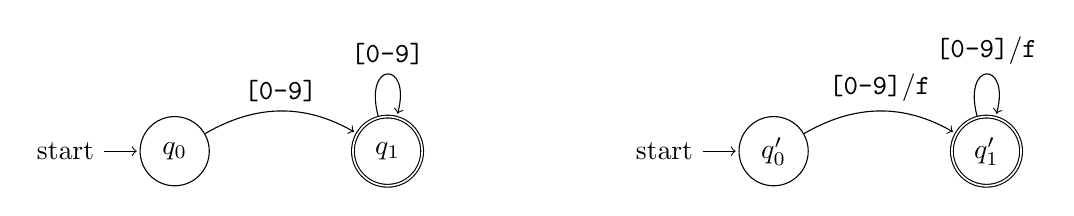
\begin{tikzpicture}[shorten >=1pt, node distance=1.8cm, auto]
  \node[state, initial] (q0)   {$q_0$}; 
  \node[state, accepting] (q1) [right=of q0] {$q_1$}; 

   \path[->] 
   (q0) edge [bend left] node {\texttt{[0-9]}} (q1)
   (q1) edge [loop above] node {\texttt{[0-9]}} (q1);

  \node[state, initial] (q0') [right=4cm of q1] {$q_0'$}; 
  \node[state, accepting] (q1') [right=of q0'] {$q_1'$}; 

   \path[->] 
   (q0') edge [bend left] node {\texttt{[0-9]}/$\texttt{f}$} (q1')
   (q1') edge [loop above] node {\texttt{[0-9]}/$\texttt{f}$} (q1');
\end{tikzpicture}
\caption{Corresponding SFA and SFT for \texttt{/[0-9]+/}}
\label{fig-snfa-pattern}
\end{figure}

\noindent\emph{Step 2.}
Figure \ref{fig-snfa-replacement} depicts the automata for the replacement string "\texttt{NUM}". The left side shows the SFA that accepts this constant string, while the right side presents its SFT transformation. The transformation employs an indexed output function \texttt{g} that emits characters of the replacement string sequentially:
\[
\texttt{g} = \lambda~i~x.~\texttt{match}~i~\texttt{with}~
\begin{cases}
1 \mapsto [(78, 78)] & \text{(ASCII for 'N')} \\
2 \mapsto [(85, 85)] & \text{(ASCII for 'U')} \\
3 \mapsto [(77, 77)] & \text{(ASCII for 'M')} \\
\_ \mapsto \texttt{None}
\end{cases}
\]
This function maps transition indices to their corresponding character outputs, using ASCII codes to represent the string "\texttt{NUM}" character by character.


\begin{figure}[h] \centering
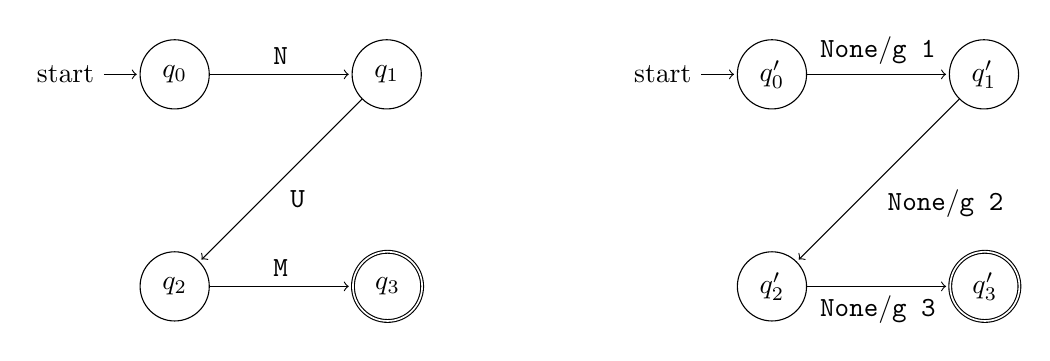
\begin{tikzpicture}[shorten >=1pt, node distance=1.8cm, auto]
  % Original NFA for "ITP"
  \node[state, initial] (q0)   {$q_0$}; 
  \node[state] (q1) [right=of q0] {$q_1$}; 
  \node[state] (q2) [below=of q0] {$q_2$}; 
  \node[state, accepting] (q3) [right=of q2] {$q_3$}; 

  \path[->] 
  (q0) edge node {\texttt{N}} (q1)
  (q1) edge node {\texttt{U}} (q2)
  (q2) edge node {\texttt{M}} (q3);

  % Duplicate NFA for "ITP" on the right
  \node[state, initial] (q0') [right=4cm of q1] {$q_0'$}; 
  \node[state] (q1') [right=of q0'] {$q_1'$}; 
  \node[state] (q2') [below=of q0'] {$q_2'$}; 
  \node[state, accepting] (q3') [right=of q2'] {$q_3'$}; 

  \path[->] 
  (q0') edge node {\texttt{None}/\texttt{g 1}} (q1')
  (q1') edge node {\texttt{None}/\texttt{g 2}} (q2')
  (q2') edge node[below] {\texttt{None}/\texttt{g 3}} (q3');
\end{tikzpicture}
\caption{Corresponding SFA and SFT for "\texttt{NUM}"}
\label{fig-snfa-replacement}
\end{figure}


\noindent\emph{Step 3.}
Figure \ref{fig-rearranged-automata} presents the complete SFT construction, obtained by composing the pattern-matching SFT (Fig. \ref{fig-snfa-pattern}) with the replacement-generating SFT (Fig. \ref{fig-snfa-replacement}). The composition process involves two key modifications:
\begin{enumerate}
  \item Connect the two SFTs by adding $\varepsilon$-transitions (labeled with \texttt{None}/\texttt{f}) from each accepting state of the pattern-matching SFT to the initial state of the replacement-generating SFT
  \item Augment the resulting transducer with self-loop transitions at both ends, labeled with $\Sigma/\texttt{f}$, where $\Sigma$ represents the full alphabet. These transitions enable the SFT to process arbitrary input prefixes and suffixes while preserving the matched substring for replacement
\end{enumerate}

\begin{figure}[h] \centering
  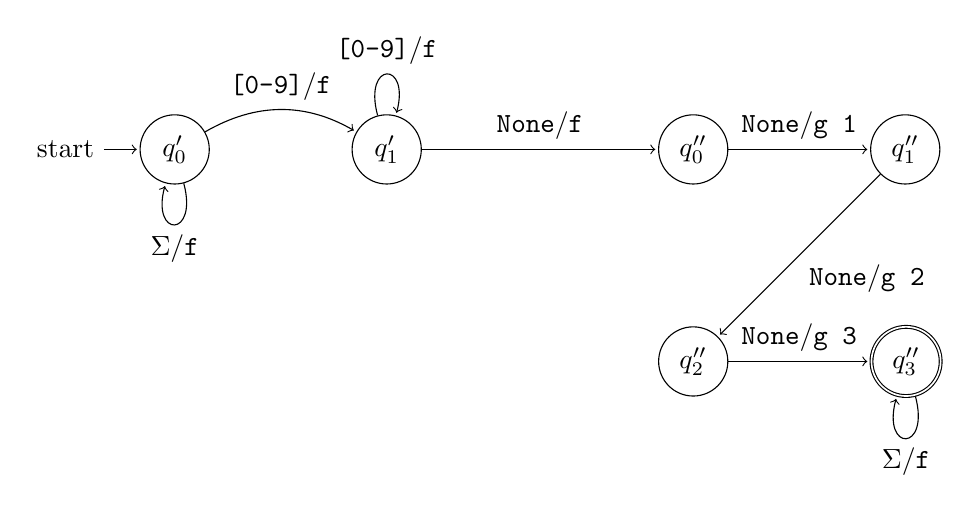
\begin{tikzpicture}[shorten >=1pt, node distance=1.8cm, auto]
    % Second automaton from the first figure
    \node[state, initial] (q0') {$q_0'$}; 
    \node[state] (q1') [right=of q0'] {$q_1'$}; 
  
     \path[->] 
     (q0') edge [bend left] node {\texttt{[0-9]}/$\texttt{f}$} (q1')
     (q1') edge [loop above] node {\texttt{[0-9]}/$\texttt{f}$} (q1')
     (q0') edge [loop below] node {$\Sigma$/$\texttt{f}$} (q0');
  
    % Second automaton from the second figure
    \node[state] (q0'') [right=3cm of q1'] {$q_0''$}; 
    \node[state] (q1'') [right=of q0''] {$q_1''$}; 
    \node[state] (q2'') [below=of q0''] {$q_2''$}; 
    \node[state, accepting] (q3'') [right=of q2''] {$q_3''$}; 
  
    \path[->] 
    (q0'') edge node {\texttt{None}/\texttt{g 1}} (q1'')
    (q1'') edge node {\texttt{None}/\texttt{g 2}} (q2'')
    (q2'') edge node {\texttt{None}/\texttt{g 3}} (q3'')
    (q3'') edge [loop below] node {$\Sigma$/$\texttt{f}$} (q3'')
    (q1') edge node {\texttt{None}/\texttt{f}} (q0'');
  \end{tikzpicture}
  \caption{The SFT for the replacement operation $\texttt{replace}(s, $\texttt{/[0-9]+/}$, $\text{NUM}$)$}
  \label{fig-rearranged-automata}
  \end{figure}


  Having constructed the SFT, we can now compute the forward image of the replacement operation. Consider the string constraint $s' = \texttt{replace}(s,~\texttt{/[0-9]+/},~\text{"}\texttt{NUM}\text{"})$, where we aim to characterize the possible values of $s'$. Let $\mathcal{T}$ denote the constructed SFT modeling the replacement operation, and let $\mathcal{A}$ be the SFA representing the domain of possible values for the input string $s$. The forward image of this replacement operation is given by the product $\mathcal{T} \times \mathcal{A}$, which precisely captures the set of all possible output strings that can be produced by applying the replacement operation to any input string accepted by $\mathcal{A}$.
  Our string solver uses this forward image to do forward propagation for further string solving.

  \emph{Comparison with SMT-LIB Semantics.} It is important to note that our formalization differs from the standard SMT-LIB semantics for the replacement operation. In SMT-LIB, the \texttt{str.replace} operation is defined to replace only the \emph{first} occurrence of a substring matching the given pattern. In contrast, our semantics allows for a more general interpretation where any matching substring may be replaced. 




\subsection{Experiments}

We have implemented CertiStrR, an extension of the Certified String Solver CertiStr \cite{cpp/KanLRS22}, to support string replacement operations\footnote{The implementation is available at \url{https://github.com/ShlKan/certified-str-solver}}. While the core solving algorithm maintains the certification guarantees of CertiStr, the frontend components are implemented using established non-certified  OCaml libraries: dolmen \cite{dolmen} for SMT-LIB parsing and ocaml-re-nfa \cite{ocaml-re-nfa} for regular expression to NFA conversion. 

CertiStrR implements two kinds of SMT-LIB's replacement operations:
\texttt{str.replace s p r}: a string-based replacement where pattern \texttt{p} is a constant string. \texttt{str.replace\_re s p r}: a regular expression-based replacement where pattern \texttt{p} is a regular expression

Listing \ref{lst-smtlib-code} demonstrates the regular expression variant through an example that replaces numeric sequences with the string "\texttt{NUM}". The constraints are satisfiable because the input string \texttt{a} = "\texttt{2024,2025}" contains a substring "\texttt{2025}" that matches the regular expression \texttt{re.+ (re.range "0" "9")} (equivalent to \texttt{/[0-9]+/}), and replacing this match with "\texttt{NUM}" yields the expected output string \texttt{b} = "\texttt{2024,NUM}".
%

As discussed in the previous subsection, our replacement semantics differs from the SMT-LIB standard semantics.
When we run the SMT solver CVC5 \cite{cvc5} with the example code in Listing \ref{lst-smtlib-code}, the result is UNSAT because CVC5 only matches the first occurrence of the pattern.


\begin{lstlisting}[language=SMTLIB, caption={Example SMT-LIB Code}, label={lst-smtlib-code}]
  (set-logic QF_S)
  (declare-fun a () String)
  (declare-fun b () String)
  (assert (= a "2024,2025"))
  (assert (= b "2024,NUM"))
  (assert (= b (str.replace_re a (re.+ (re.range "0" "9")) "NUM")))
  (check-sat)
  \end{lstlisting}


  We evaluate CertiStrR using benchmarks from SMT-LIB 2024 \cite{smtlib_benchmarks}, focusing on the QF\_S and QF\_SLIA logic fragments. The benchmarks are divided into two categories based on the replacement operations: (1) string-based replacement (\texttt{str.replace}) and (2) regular expression-based replacement (\texttt{str.replace\_re}). Due to CertiStrR's current front-end limitations in supporting the full SMT-LIB specification, we preprocess certain operations. For instance, conjunctive assertions of the form \texttt{(assert (and c1 c2))} are decomposed into separate assertions \texttt{(assert c1)} and \texttt{(assert c2)} when \texttt{c1} and \texttt{c2} are string constraints supported by CertiStrR.

% replace_re
% Average real time: 0.37 seconds
% Total number of real entries: 98
% Average user time: 0.35 seconds
% Total number of user entries: 98
% Average sys time: 0.01 seconds
% Total number of sys entries: 98
% Total number of SAT entries: 61
% Total number of UNSAT entries: 4
% Total number of inconclusive entries: 30

% replace_str   
% Average real time: 0.27 seconds
% Total number of real entries: 323
% Average user time: 0.25 seconds
% Total number of user entries: 323
% Average sys time: 0.01 seconds
% Total number of sys entries: 323
% Total number of SAT entries: 315
% Total number of UNSAT entries: 173
% Total number of inconclusive entries: 8


\begin{table}[h]
  \centering
  \begin{tabular}{lccccc}
      \toprule
      & \textbf{SAT} & \textbf{UNSAT} & \textbf{Inconclusive} & \textbf{Time} & \textbf{Number of Tests} \\
      \midrule
      \texttt{replace\_str} & 142 & 173 & 8 & 0.27 & 323\\
      \texttt{replace\_re} & 57 & 4 & 30 & 0.37 & 98\\
      \bottomrule
  \end{tabular}
  \caption{Performance metrics for string operations}
  \label{tab:string_operations}
\end{table}

The experimental evaluation was conducted on a laptop with an Apple M4 processor and 24 GB of memory, with a time limit of one minute per test. 
The results show average execution times of 0.27 seconds for \texttt{str.replace} and 0.37 seconds for \texttt{str.replace\_re} operations. Test outcomes were classified into three categories: SAT (satisfiable), UNSAT (unsatisfiable), and Inconclusive.
%
An "Inconclusive" result indicates that the solver cannot determine satisfiability, not due to timeout but rather due to inherent limitations of the forward-propagation algorithm inherited from CertiStr \cite{cpp/KanLRS22}. Specifically, when the string constraints do not satisfy the tree property, the forward-propagation algorithm may be unable to reach a definitive conclusion, even when the variable domains remain non-empty after propagation.



Our performance analysis revealed that while the SFT-based replacement operation modeling is efficient, the primary computational bottleneck stems from automata accumulation during forward-propagation. Consider the following constraint system:
\[
x = x_1\texttt{++}x_2;~x = \texttt{replace}(x_3, p, r);~x = x_4;~x = \texttt{replace}(x, p_1, r_1);
\]
where \texttt{++} denotes string concatenation. The variable $x$ appears multiple times on the left-hand side of the equations, causing the forward-propagation algorithm to accumulate automata representations for each constraint: $x_1\texttt{++}x_2$, \texttt{replace}($x_3, p, r$), $x_4$, and \texttt{replace}($x, p_1, r_1$). Each accumulation step requires computing the product of the current automaton with the previous result. Given that the product operation has a worst-case complexity of $O(n^2)$, where $n$ represents the automaton size, this repeated accumulation can lead to state and transition explosion.


\subsection{Effort of Certified Development}

We discuss the effort of certified SFT development in this subsection.
Table \ref{tab:abstract_impl} provides an overview. The abstract-level development means all formalizations in Section \ref{sec:product-operation}. The implementation-level development means all formalizations in Section \ref{sec_alg_refinement}.

\begin{table}[h]
  \centering
  \begin{tabular}{lccc}
      \toprule
      & \textbf{Definitions} & \textbf{Lemmas} & \textbf{Proofs} (lines of code) \\
      \midrule
      Abstract & & & \\
      Implementation & & & \\
      \bottomrule
  \end{tabular}
  \caption{Overview of the effort of certified development}
  \label{tab:abstract_impl}
\end{table}


\section{Related Work}
\label{sec:related-work}


\section{Conclusion}
\label{sec:conclusion}


\bibliography{literature}
\end{document}